\section{Feature detection (new title TBD)}  \label{sec:features}

\begin{figure}
    \centering
    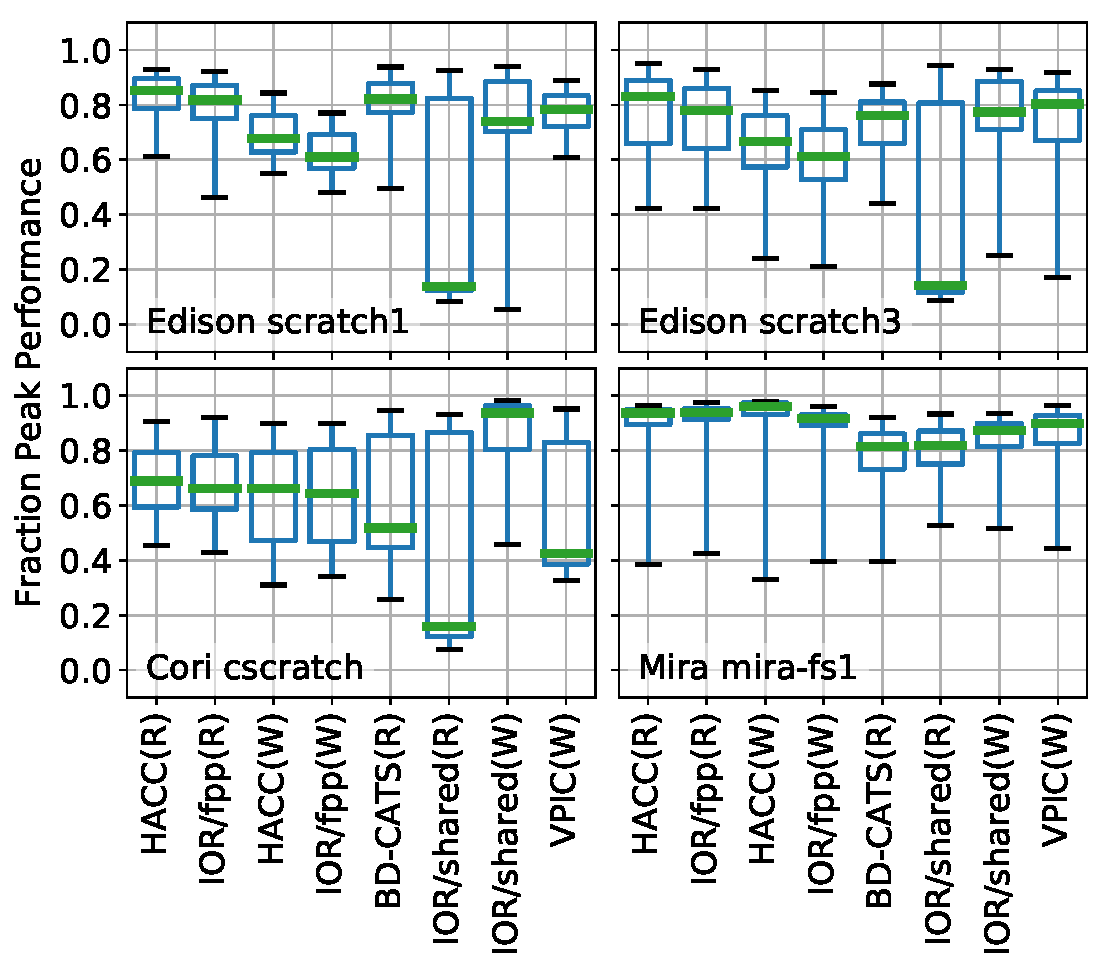
\includegraphics[width=0.9\columnwidth]{summary-boxplots}
    \vspace{-.15in}
    \caption{I/O performance grouped by test applications and read(R)/write(W) mode.  Whiskers represent the 5th and 95th percentiles.}
    \label{fig:summary-boxplots}
%   \vspace{-.3in}
\end{figure}


\begin{figure*}
    \centering
    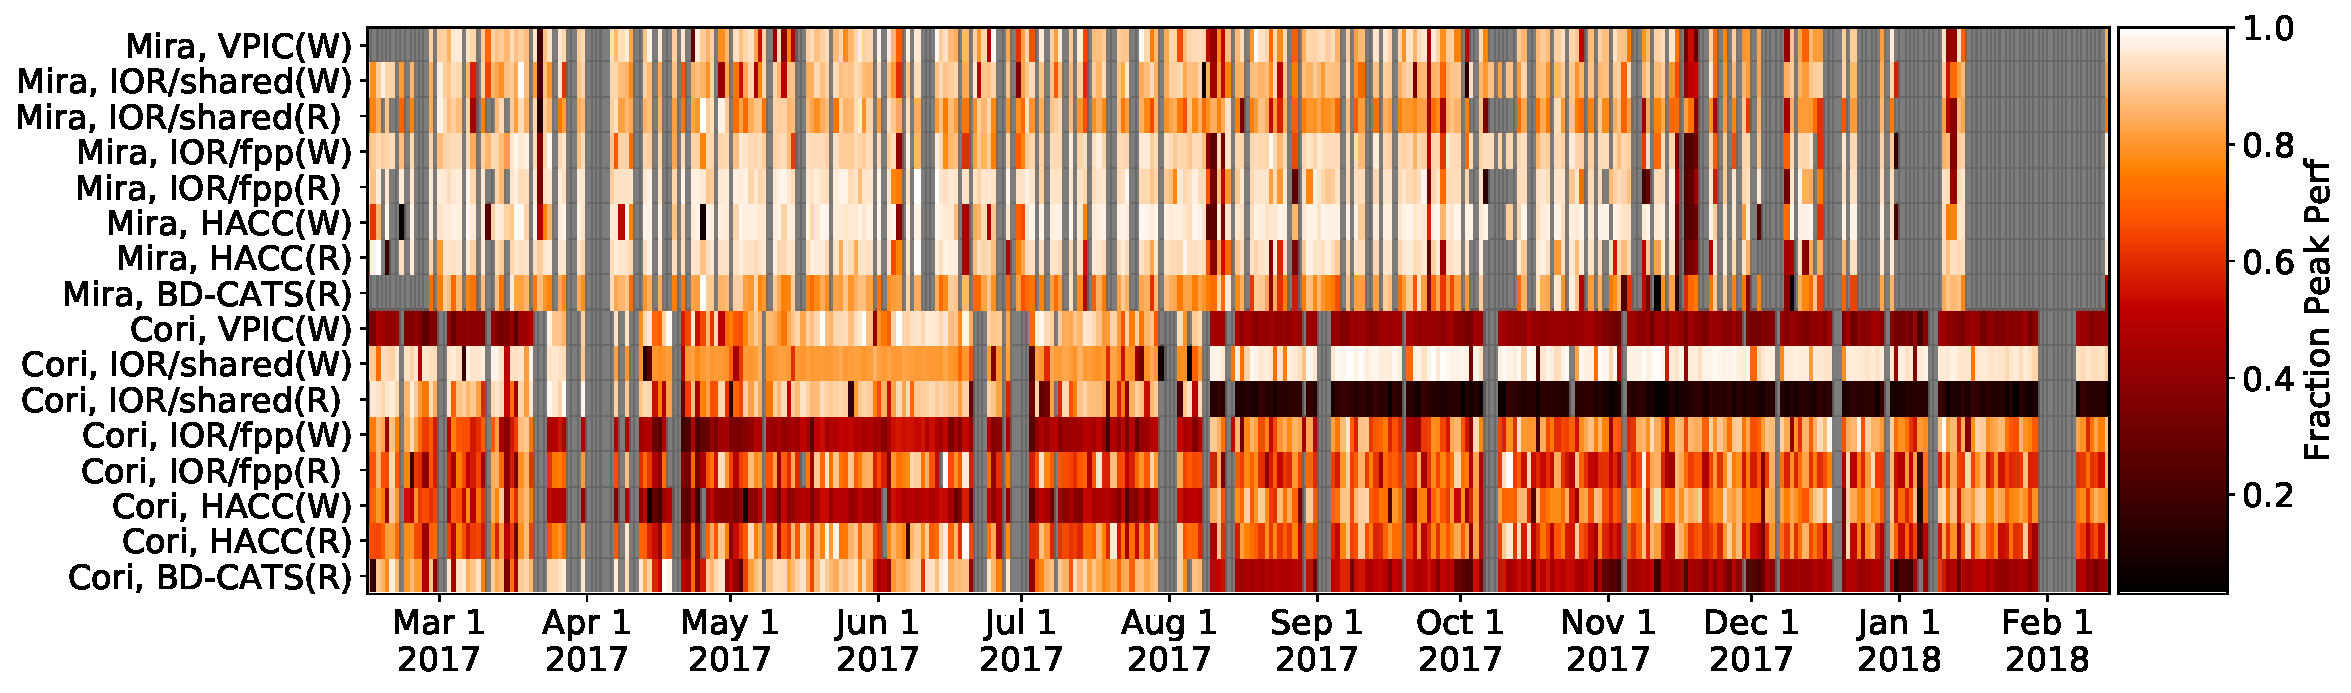
\includegraphics[width=0.90\linewidth]{summary-heatmap}
    \vspace{-.2in}
    \caption{Performance of daily benchmarks normalized to each benchmark's peak observed performance on the specified storage system.  The y-axis labels show combinations of system, I/O motif, and mode (Read/Write).  Grey represents days on which no observations were made.  The two regions highlighted in green boxes are expanded upon in Figure \ref{fig:regions-heatmap}.}
    \label{fig:summary-heatmap}
\end{figure*}

\begin{figure}
    \centering
    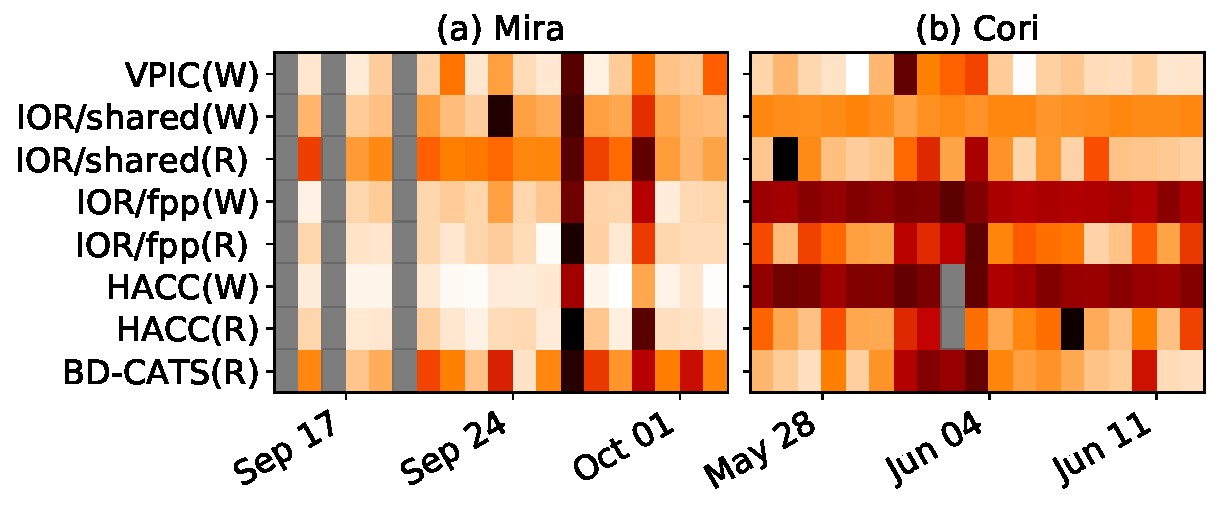
\includegraphics[width=0.90\linewidth]{regions-heatmap}
    \vspace{-.2in}
    \caption{Examples of structure in the fraction of peak performance observations.  Color scale is the same as that in Figure \ref{fig:summary-heatmap}.  In (a), the vertical band on Sept 26 corresponds to a transient system-wide degradation on \mira.  The horizontal bands for the IOR file-per-process write workload (IOR/fpp(W)) and HACC write workload (HACC(W)) in (b) show a sustained performance problem for file-per-process write workloads on \cori.}
    \label{fig:regions-heatmap}
\end{figure}

\subsection{Statistical Summary} \label{sec:features/summary}

% \TODO{Things that are important here: behavior over time, grouping data sources in a way that helps understand scope, focusing on fundamental \emph{changes} in performance rather than steady state, everything in one view.}

I/O performance is known to vary as a function of (a) application I/O pattern, (b) whether I/Os read or write, and (c) the architecture of the system on which I/O is happening~\cite{Lockwood2017, Xie2012}.
To remove the effects of these factors and enable us to focus on performance \emph{variation}, we therefore express the performance of each of the 11,986 observations in terms of its \emph{fraction of peak performance}.
This fraction of peak performance is defined as the absolute performance (in bytes/sec) of an observation divided by the maximum absolute performance observed across all jobs with a common (a), (b), and (c) above.

The distribution of the fraction of peak performance measurements for four of the five systems tested is shown in Fig. \ref{fig:summary-boxplots} and demonstrates that the performance of active I/O performance probes on production file systems is highly dynamic.
Further decomposition of two of these performance distributions is shown in Fig. \ref{fig:summary-heatmap} and reveals that performance variation is not randomly distributed over the year.
A significant amount of time-correlated structure, highlighted in Fig. \ref{fig:summary-heatmap}, demonstrates three phenomena commonly observed:

\begin{enumerate}[leftmargin=*]
\item Dark vertical bands, exemplified in the \mira data in Fig. \ref{fig:regions-heatmap}, represent transient system-wide issues that resulted in a uniform loss of performance for all applications tested that day.
\item Dark horizontal bands, shown in the \cori data, indicate a long-term degradation in performance that disproportionately affects a specific I/O motif or reads or writes.
\item Isolated dark blocks represent individual application runs where performance was poor despite an absence of system-wide transients (vertical bands) or systematic, motif-specific problems (horizontal bands).
\end{enumerate}

% \TODO{Insert some smooth one-sentence transition into next section; perhaps mention that we don't consider the aforementioned results as surprising and the best is yet to come.} DONE - 2018-03-25 gkl

The preponderance of these time-correlated phenomena underscore the need to consider variation as a function of time.
What may qualify as abnormally poor performance during one part of the year may be the baseline expected performance during another, and being able to understand these different regions of performance and variation is essential toward identifying and remedying their root causes.
It is therefore imperative to have a systematic approach towards identifying different regions of I/O performance to differentiate long-term performance degradation from shorter-term and transient variation.
In the following section, we describe a general approach to address this problem of partitioning performance measurements into regions of significant performance trends.

\TODO{In addition to above, maybe worth pointing out this is only showing results based on Darshan data, so we haven't even crossed into holistic territory, where datasets become much larger and difficult to analyze. -SS}

\TODO{Need to add definition of coverage factors somewhere}




\subsection{Time-dependent Analysis} \label{sec:features/timedependent}

\begin{figure}[t]
    \centering
    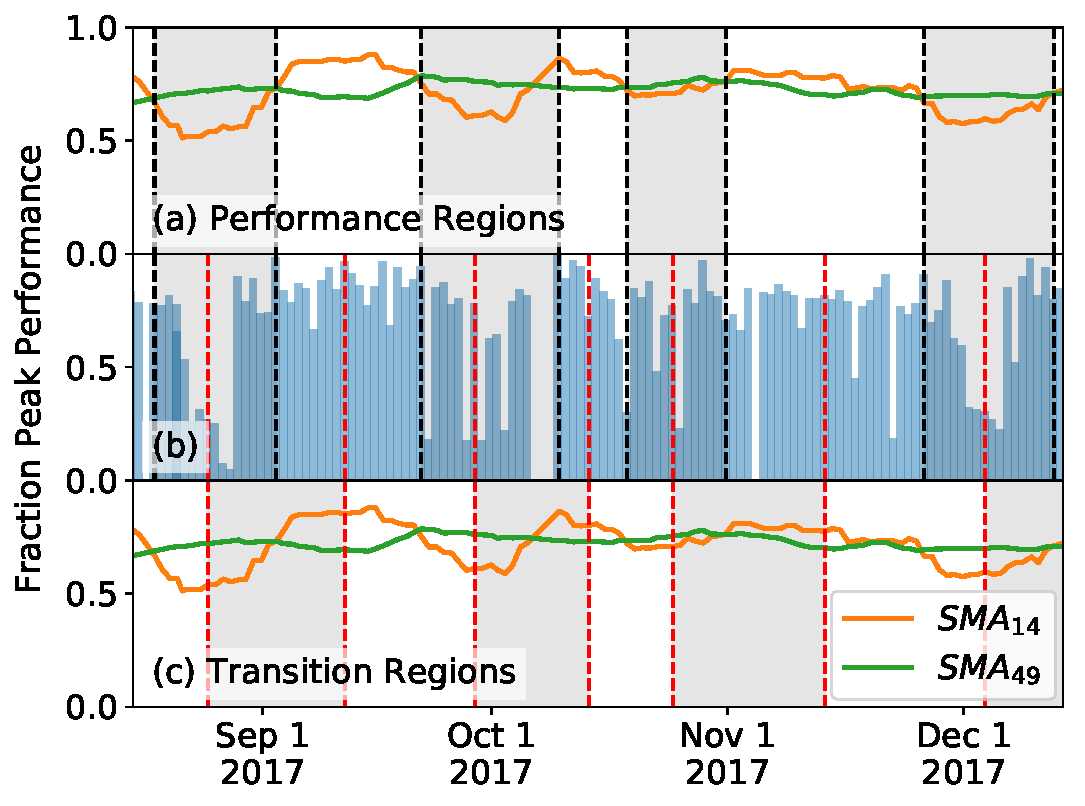
\includegraphics[width=1.0\columnwidth]{segment-explain}
    \vspace{-.35in}
    \caption{Example of overlaying two simple moving averages (SMAs) to identify (a) \emph{divergence regions} and (c) \emph{trend regions} in the \edison \scratchtwo IOR/fpp write dataset.  Middle pane (b) includes raw performance measurements (blue bars) with both SMA crossovers (black dashed lines) and divergence region centroids (red dashed lines).}
    \label{fig:segment-explain}
    % source: sc18_segments-explain.ipynb
\end{figure}

The data in Fig. \ref{fig:summary-heatmap} demonstrates that nominally optimal I/O performance for a given system evolves over time.
As a result, it is often not meaningful to express the performance of an application as being good or bad with respect to an absolute peak performance;
rather, "bad" performance (and its causes) should be classified with respect to what qualifies as "good" performance for a timescale of interest.
To address this issue, we propose applying Simple Moving Averages (SMAs) as a means to identify correlated performance trends in production parallel file systems.
This approach has commonly been applied in the context of financial market technical analysis, where moving averages are used to attenuate the day-to-day volatility in the price movements of underlying assets and to help identify larger trends in these movements~\cite{james1968monthly,gunasekarage2001profitability}.

Given a time window of width $w$, we define the SMA for a metric $M$ at time $t$ as the average value of $M$ over ${-0.5w <= t < +0.5w}$;
when chosen to be sufficiently wide ($w = 49$ days), the resulting $\textup{SMA}_{long}$ provides a rapid visual means to identify performance degradation or recovery that lasts for $O(\textup{weeks})$.
Superimposing a second SMA with a shorter window ($w = 14$ days), such as $\textup{SMA}_{short}$, then allows us to distinguish short-term performance anomalies that last for $O(\textup{days})$ from longer-term performance evolution.
We found the exact choice of $w_{short}$ and $w_{long}$ to be somewhat arbitrary; adjusting these values by as much as $\pm 50\%$ did not affect the identification of the most significant events presented here.
In addition, a specific choice of $w$ does not preclude analyzing events longer or shorter than $w$, and we demonstrate methods to address this in Sections \ref{sec:results/longterm} and \ref{sec:results/shortterm}.

In the following analysis, we apply this SMA-based approach to procedurally identify and classify performance variation at all time scales, ranging from long-term system health issues to transient performance loss due to probabilistic contention.


%We define $\textup{SMA}_{short}$ and $\textup{SMA}_{long}$ as simple moving averages of widths $w_{short}$ and $w_{long}$, and for this study, chose $w_{short} = 14$ days and $w_{long} = 49$ days as a reasonable choice to focus on correlated performance events that occurred over $O(\textup{weeks})$.

% J_{app, rw, sys}
After calculating $\textup{SMA}_{short}$ and $\textup{SMA}_{long}$ for each of the set of performance observations $J_{app, rw, sys}$, we identify \emph{divergence regions}. These are defined as non-overlapping subsets of $J_{app, rw, sys}$ that are bounded by the crossover points between $\textup{SMA}_{long}$ and $\textup{SMA}_{short}$.
SMA crossover points are, again, a popular tool in technical analysis of financial markets, used to detect trend shifts in asset prices, often for predictive purposes\footnote{Though we note that the predictive capability of SMA crossovers is a source of controversy even in the financial community, and thus, we focus solely on using them as tools for managing volatility and detecting trends in historical datasets.} (e.g., as signals to buy or sell an asset based on the direction of the short and long-term SMAs at the time they crossover)~\cite{brock1992simple}.
Figure \ref{fig:segment-explain}a illustrates this partitioning of the IOR/fpp write workload measurements on \edison's \scratchtwo file system;
dashed lines represent the crossover points of $\textup{SMA}_{long}$ and $\textup{SMA}_{short}$, and divergence regions are shaded in alternating gray and white.
As Figure \ref{fig:segment-explain}a illustrates, using SMA crossovers to identify divergence regions results in temporally contiguous subsets of performance measurements that capture a period of time with consistently good (${\textup{SMA}_{short} > \textup{SMA}_{long}}$) or bad (${\textup{SMA}_{short} < \textup{SMA}_{long}}$) performance.

Figure~\ref{fig:segment-explain}a shows 8 distinct divergence regions, but does not provide any insight into the causes of the transitions. To understand the causes of these transitions, we also partition $J_{app, rw, sys}$ into \emph{trend regions}.
For each divergence region, we identify the temporally center-most observation as the centroid of that region, as illustrated in Figure \ref{fig:segment-explain}b, as red dashed lines.
We then define trend regions as those regions bounded by centroids (Figure \ref{fig:segment-explain}c), and each trend region overlaps with exactly two divergence regions and vice versa.
The principal difference between the two is that divergence regions contain observations that are uniformly good or uniformly bad, and trend regions capture performance transitioning from bad to good or vice versa. Divergence regions are used to group measurements which are similar, trend regions are used to understand the reasons for transition between different performance regimes.

\TODO{Can we say more here about what we learned from Figure 3?}


